\chapter{Applications, Limitations, and Future Work}\label{ch:future}

\section{Application Opportunities}
Potential deployments include industrial exhaust heat recovery, automotive thermal scavenging, and remote sensor powering where thermal sources fluctuate.

A mission-level energy metric is
\begin{equation}\label{eq:mission_energy}
E_{mission}=\int_{0}^{t_f} P(t)\,\mathrm{d}t.
\end{equation}

\section{Validation Strategy}
A defense-ready validation plan includes:
\begin{itemize}
    \item DSC for latent heat and phase interval verification,
    \item SEM for pore architecture and filler dispersion,
    \item four-probe conductivity for $\sigma_{eff}$,
    \item laser flash or transient plane source methods for $k_{eff}$,
    \item accelerated thermal cycling for durability and leakage metrics.
\end{itemize}

Measurement uncertainty propagation is estimated by
\begin{equation}\label{eq:uncertainty}
u_Y^2\approx\sum_i\left(\frac{\partial Y}{\partial x_i}\right)^2\nu_{x_i}^2.
\end{equation}

\section{Limitations}
Key limitations are long-term humidity sensitivity of PVA, potential nanofiller aggregation beyond optimal loading, and manufacturability challenges for module-scale consistent pore topology.

\section{Future Work Roadmap}
Future work should integrate humidity-barrier strategies, multiscale tomography-informed digital twins, and pilot-scale manufacturing.

\begin{figure}[htbp]
\centering
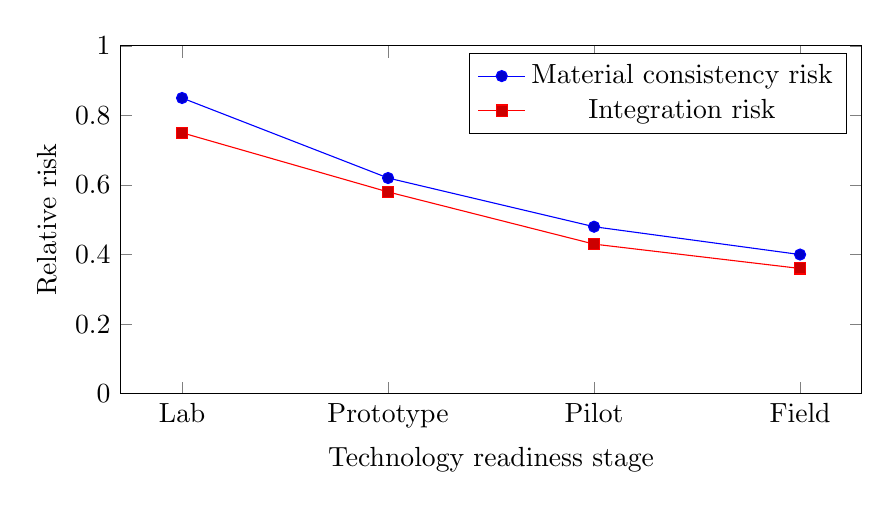
\begin{tikzpicture}
\begin{axis}[width=11cm,height=6cm,xlabel={Technology readiness stage},ylabel={Relative risk},symbolic x coords={Lab,Prototype,Pilot,Field},xtick=data,ymin=0,ymax=1.0]
\addplot+[mark=*] coordinates {(Lab,0.85)(Prototype,0.62)(Pilot,0.48)(Field,0.40)};
\addplot+[mark=square*] coordinates {(Lab,0.75)(Prototype,0.58)(Pilot,0.43)(Field,0.36)};
\legend{Material consistency risk,Integration risk}
\end{axis}
\end{tikzpicture}
\caption{Indicative risk evolution during scale-up.}
\label{fig:future_risk}
\end{figure}

\begin{table}[htbp]
\centering
\caption{Proposed experimental validation matrix.}
\label{tab:validation_matrix}
\begin{tabular}{lll}
\toprule
Objective & Method & Output \\
\midrule
PCM latent behavior & DSC & $L$, $T_m$, hysteresis \\
Scaffold morphology & SEM & Pore size, continuity, filler dispersion \\
Electrical transport & Four-probe test & $\sigma_{eff}(T)$ \\
Thermal transport & TPS / Laser flash & $k_{eff}(T)$ \\
Cycling durability & Thermal shock cycling & $\Lambda_N$, $D_N$ \\
\bottomrule
\end{tabular}
\end{table}

\begin{table}[htbp]
\centering
\caption{Roadmap milestones for future development.}
\label{tab:future_roadmap}
\begin{tabular}{p{3.5cm}p{8cm}}
\toprule
Time horizon & Milestone \\
\midrule
0--1 year & Lab-scale prototype with calibrated DSC/SEM/transport datasets \\
1--3 years & Module-level integration with humidity barrier and encapsulation optimization \\
3--5 years & Pilot manufacturing and techno-economic benchmarking \\
\bottomrule
\end{tabular}
\end{table}
